\chapter{Część kliencka rozszerzenia}
W przypadku edytora Visual Studio Code, komunikacja między serwerem LSP a edytorem następuje poprzez dodatkowy adapter w postaci osobnego małego rozszerzenia. Dodatkowo, nie wszystkie możliwości edytora są wspierane przez protokół. Część kliencka rozszerzenia zatem ma 2 funkcjonalności:

\begin{enumerate}
    \item Uruchomienie serwera i komunikacja z nim.
    \item Udostępnienie funkcjonalności które nie są wspierane przez protokół LSP.
\end{enumerate}

\section{Komunikacja z serwerem}
Ponieważ zarówno klient jak i serwer LSP są napisane w środowisku Node.js, możliwe było wykorzystanie bibliotek udostępnionych przez twórców edytora, przez co nawiązanie połączenia i jego obsługa ogranicza się do wskazania pliku serwera. Dodatkowo moduł serwera zostaje przy utworzeniu dodany do listy obiektów usuwanych przy zamknięciu rozszerzenia (np. zamknięte zostały wszystkie pliki Lua lub został wyłączony edytor).

\section{Dodatkowe funkcjonalności}
Klient poza przekazywaniem pracy do serwera, może implementować wiele osobnych funkcjonalności. Są to między innymi rejestracja danego języka programowania w słowniku edytora, co pozwala wielu wtyczkom dotyczących jednego języka na korzystanie ze swoich funkcji nawzajem. Inną ważną funkcjonalnością jest dodanie opisu kolorowania składni. W przypadku VS Code robi się to przez załączenie pliku gramatyki dla edytora TextMate (podejście identyczne jak w przypadku rozszerzeń do edytora Atom). Przykładowo reguła składni:
\pagebreak

\begin{lstlisting}[language=XML, morekeywords={dict,key,string}]
    <dict>
        <key>match</key>
        <string>(?&lt;![\w\d.])\d+(?![pPeE.0-9])</string>
        <key>name</key>
        <string>constant.numeric.integer.lua</string>
    </dict>
\end{lstlisting}

Spowoduje, że fragmentom tekstu pasującym do podanego wyrażenia regularnego (w tym przypadku liczbom całkowitym w systemie dziesiętnym) zostanie przypisana etykieta \texttt{constant.numeric.integer}, która zostanie odpowiednio pokolorowana na podstawie wybranego przez użytkownika motywu kolorystycznego. W przypadku prezentowanego motywu:

\begin{lstlisting}[language=XML, morekeywords={dict,key,string}]
    <dict>
        <key>name</key>
        <string>Number</string>
        <key>scope</key>
        <string>constant.numeric</string>
        <key>settings</key>
        <dict>
            <key>foreground</key>
            <string>#AE81FF</string>
        </dict>
    </dict>
\end{lstlisting}

wszystkie fragmenty tekstu, których etykieta zawiera prefiks \texttt{constant.numeric} zostaną pokolorowane na kolor fioletowy.

\begin{figure}[H]
\centering
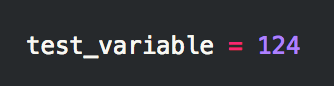
\includegraphics{Chapters/kolorowanie_skladni}
\end{figure}
